%        File: hw1.tex
%     Created: Sat Apr 06 10:00 AM 2013 P
% Last Change: Sat Apr 06 10:00 AM 2013 P
%
\documentclass[11pt]{article}

\usepackage{amsmath, amssymb, amsthm, cite, graphicx, float, mathrsfs, commath, dsfont, bbm, bm}
\usepackage[mathscr]{eucal}
\usepackage[sc]{mathpazo}
\linespread{1.05}
%\usepackage{setspace}
%\onehalfspacing
\usepackage[margin=1in, top=.8in, left=.8in]{geometry}
\usepackage{color}

% new commands
\DeclareMathOperator*{\argmin}{arg\,min}
\DeclareMathOperator{\sgn}{sgn}
\newcommand{\E}{\mathrm{E}}
\newcommand{\Var}{\mathrm{Var}}
\newcommand{\Cov}{\mathrm{Cov}}
\newcommand{\Cor}{\mathrm{Cor}}
\newcommand{\id}{\operatorname{id}}
\newcommand{\diag}{\operatorname{diag}}
\newcommand{\Id}{\operatorname{Id}}
\newcommand{\tr}{\operatorname{tr}}
\newcommand{\Q}{\mathbb{Q}}
\newcommand{\C}{\mathbb{C}}
\newcommand{\R}{\mathbb{R}}
\newcommand{\Z}{\mathbb{Z}}
\newcommand{\F}{\mathbb{F}}
\newcommand{\N}{\mathbb{N}}

\newcommand{\indep}{\rotatebox[origin=c]{90}{$\models$}}

% 524 commands
%\newcommand{\norm}[1]{\| #1 \|}
\DeclareMathOperator{\spn}{span}
%\newcommand{\spn}{\operatorname{span}}
\newcommand{\onenorm}[1]{\| #1 \|_{L^1(\mathbb R^d)}}
\newcommand{\twonorm}[1]{\| #1 \|_{L^2(\mathbb R^d)}}

% 534 commands
\renewcommand{\Re}{\text{Re\,}}
\renewcommand{\Im}{\text{Im\,}}

\begin{document}
\pagestyle{empty}
\hfill Abraham Engle

\hfill Stat 571

\hfill \today
\\Following the notation in Jon's book, I let $J_n$ denote the $n\times n$ matrix of all ones, and I use both facts that
	\begin{align*}
		(aI_n+bJ_n)^{-1} &= \frac{1}{a}\left(I_n - \frac{b}{a+nb}J_n \right), a\neq 0, a+nb\neq 0 \\
		\det(aI_n + bJ_n) &=  a^{n-1}(a+nb)
	\end{align*}
The first follows from the Sherman-Morrison-Woodbury formula for finding the inverse of a matrix after a rank one update (in this case, $b\bm{1}\bm{1}^T=bJ_n$). The second from the matrix determinant lemma applied to the rank one update.
\begin{enumerate}
    %1
	\item The marginal distribution for each $i=1,2,\dotsc,n$ is
	\[ 
		Y_i \sim_{indp} N_{n_i}\left(\beta_0\bm{1}_{n_i},\Sigma_i\right),
	\]
	where $\Sigma_i = \begin{pmatrix}
		\sigma^2_Y + \sigma^2_a & \sigma^2_a & \cdots & \sigma^2_a \\
		\sigma^2_a & \sigma^2_Y + \sigma^2_a & \cdots & \sigma^2_a\\
		\vdots & \vdots & \ddots & \vdots \\
		\sigma^2_a & \sigma^2_a & \cdots & \sigma^2_Y + \sigma^2_a
	\end{pmatrix}\in \R^{n_i\times n_i}$. For sufficiency, we rely on cluster independence from the assumptions of the problem and thus have
	\[
		Y:=\begin{pmatrix}
			Y_1 \\ Y_2 \\ \vdots \\ Y_n
		\end{pmatrix} \sim N_{\sum_{i=1}^n n_i} \left(\beta_0 \bm{1}_{\sum n_i}, \mathrm{diag}(\Sigma_i)\right),
	\]
	From independence of clusters, the joint density is
	\begin{align*}
		f(\bm{y}_1,\dotsc,\bm{y}_n) &= \prod_{i=1}^n \frac{1}{(2\pi)^{n_i/2}}\frac{1}{\sqrt{\det\Sigma_i}}\exp\left\{-\frac{1}{2}(\bm{y}_i - \beta_0\bm{1}_{n_i})^T\Sigma_i^{-1}(\bm{y}_i-\beta_0\bm{1}_{n_i}) \right\} \\
		&= \frac{1}{(2\pi)^{\sum_i n_i/2}}\frac{1}{\sqrt{\det[\diag(\Sigma_i)]}}\exp\left\{-\frac{1}{2}\sum_{i=1}^n(\bm{y}_i - \beta_0\bm{1}_{n_i})^T\Sigma_i^{-1}(\bm{y}_i - \beta_0\bm{1}_{n_i})\right\}.
	\end{align*}
	The two terms in front of the exponential are not a problem for determining sufficiency from the Neyman-Fisher factorization. Using the inverse formula above, the quadratic form inside the exponential is
	\begin{align*}
		-\frac{1}{2}\sum_{i=1}^n(\bm{y}_i - \beta_0\bm{1}_{n_i})^T\Sigma_i^{-1}(\bm{y}_i - \beta_0\bm{1}_{n_i}) &= -\frac{1}{2\sigma_Y^2} \sum_{i=1}^n (\bm{y}_i - \beta_0\bm{1}_{n_i})^T\left(I_{n_i} - \frac{\sigma_a^2}{\sigma_Y^2 + n_i\sigma_a^2}J_{n_i}\right)(\bm{y}_i - \beta_0\bm{1}_{n_i}) \\
		&= -\frac{1}{2\sigma_Y^2} \sum_{i=1}^n y_i^Ty_i - 2\beta_0\bm{y}_i^+ + \beta_0^2n_i - \frac{\sigma_a^2}{\sigma_Y^2 + n_i\sigma_a^2}\left([\bm{y}_i^+]^2 - 2\beta_0n_i \bm{y}_i^+ + \beta_0^2 n_i^2\right),
	\end{align*}
	where $\bm{y}_i^+ := \sum_j y_{ij}$. From this decomposition of the quadratic form, define the sufficient statistics to be
	\[
		T(\bm{y}_1,\dotsc,\bm{y}_n) = ( \sum_{i,j}y_{ij}^2, \bm{y}_1^+,\dotsc,\bm{y}_n^+)
	\]
	\\ \\In terms of the sufficient statistics, we compute the expectation of the following inner product, using the formula for the expectation of a quadratic form (I show that this quantity is in terms of the sufficient statistics at the very end of the problem). Let $\overline{Y} = \frac{1}{\sum_i n_i}\sum_{i,j}y_{ij}$ and let $Y$ denote the stacked vector of observations. The quantity of interest is
	\begin{align*}
		E[(Y-\overline{Y}\bm{1})^T(Y-\overline{Y}\bm{1})] &= \tr(\Var(Y-\overline{Y}\bm{1})).
	\end{align*}
	The variance is $\Var(Y) - 2\Cov(Y,\overline{Y}\bm{1}) + \Var(\overline{Y}\bm{1})$. The first term we already know is $\diag(\Sigma_i)$. The last term is $\bm{1}\Var(\overline{Y})\bm{1}^T$, and
	\[
		\Var(\overline{Y}) = \frac{1}{(\sum n_i)^2}\bm{1}^T\diag\Sigma_i\bm{1} = \frac{1}{(\sum_i n_i)^2} \sum_{i=1}^n n_i(\sigma_a^2+\sigma_Y^2) + n_i(n_i-1)\sigma_a^2.
	\]
	We only need the trace of the covariance term, which is
	\begin{align*}
		\tr(\Cov(Y,\bm{1}\overline{Y})) &= \sum_{i,j} E[(Y_{ij}-\beta_0)(\overline{Y}-\beta_0)] \\
		&= \sum_{i,j} E[Y_{ij}\overline{Y}]  - \frac{\beta_0^2}{\sum_i n_i} \\
		&= \frac{1}{\sum_i n_i}\sum_{i,j} \sigma^2_Y + \sigma^2_a + \beta_0^2  + n_i(n_i-1) \sigma_a^2 - \beta_0^2 \\
		&= \frac{1}{\sum_i n_i}\sigma_Y^2 \sum_i n_i  + \sigma^2_a \sum_{i,j} n_i(n_i-1) + 1 \\
		&= \sigma_Y^2 + \sigma_a^2 \frac{\sum_i n_i^2}{\sum_i n_i}.
\	\end{align*}
The other two traces give
	\begin{align*}
		\tr(\Var(Y-\overline{Y}\bm{1})) &= \sum_i n_i(\sigma^2_Y + \sigma^2_a) -2(\sigma_Y^2 + \sigma_a^2 \frac{\sum_i n_i^2}{\sum_i n_i}) + \frac{1}{\sum_i n_i} \sum_{i=1}^n n_i(\sigma_a^2+\sigma_Y^2) + n_i(n_i-1)\sigma_a^2 \\
		&= (\sigma^2_Y + \sigma^2_a)\sum_i n_i - 2\sigma^2_Y - 2\sigma^2_a \frac{\sum_i n_i^2}{\sum_i n_i} + \sigma_Y^2 + \sigma_a^2 + \sigma^2_a\frac{\sum_i n_i^2}{\sum_i n_i} - \sigma_a^2 \\
		&= \sigma_a^2\sum_i n_i + \sigma_Y^2[(\sum_i n_i) - 1] -\sigma_a^2 \frac{\sum_i n_i^2}{\sum_i n_i} \\
		&= \sigma_a^2 \frac{(\sum_i n_i)^2 - \sum_i n_i^2}{\sum_i n_i} + \sigma_Y^2[(\sum_i n_i) - 1]
	\end{align*}
	Next, since 
	\[
		E[\sum_{i,j}Y_{ij}^2]=(\beta_0^2 + \sigma_a^2 + \sigma_Y^2)\sum_i n_i,
	\] and since 
	\[
		E[(\sum_j y_{ij})^2] = E[\sum_j y_{ij}^2] + \sum_{j\neq j'}E[Y_{ij}Y_{ij'}] = n_i(\sigma_a^2 + \sigma_Y^2 + \beta_0^2) + n_i(n_i-1)(\beta_0^2 + \sigma_a^2) = n_i\sigma_Y + n_i^2 \sigma_a^2 + n_i^2 \beta_0^2,
	\] if we let
	\[
		\widehat{\theta}_i = \frac{\frac{n_i^2}{\sum_i n_i} \sum_{i,j}Y_{ij}^2-(\sum_j y_{ij})^2}{n_i^2-n_i},
	\]
	then we have an unbiased estimator of $\sigma_Y^2$, which we can use along with the inner product above to define a family of unbiased estimators of $\sigma_a^2$ as follows:
	\[
		\widehat{\sigma}_a^2 = \frac{(Y-\overline{Y}\bm{1})^T(Y-\overline{Y}\bm{1}) - [(\sum_i n_i) - 1]\widehat{\theta}_i}{\frac{(\sum_i n_i)^2 - \sum_i n_i^2}{\sum_i n_i}},
	\]
	so for any choice of $i$, we obtain an unbiased estimator of $\sigma^2_a$, so the statistics cannot be complete. By reordering the clusters, suppose without loss that $n_1\neq n_2$. The above discussion produces two estimators above $g_1\neq g_2$ so that
	\[
		E[g_1(T(Y))-g_2(T(Y))] = 0,
	\]
	so does not depend on the parameters. If the statistics were complete, we would require $g_1= g_2$, which violates the completeness condition by our construction.
	\\ \\
	To finish up, we need to verify that the inner product given above is in terms of the sufficient statistics. The inner product is $Y^TY - 2\overline{Y}\bm{1}^TY + \overline{Y}^2\sum_i n_i = Y^TY - \overline{Y}^2 \sum_i n_i$. The first summand is the first statistic we defined. The second term is
	\[
		\overline{Y}^2\sum_i n_i = (\sum_i n_i)^{-1}\bm{1}^TY\bm{1}^TY = (\sum_i n_i)^{-1}\left(\bm{1}_n^T\begin{pmatrix}
			y_1^+ \\ \vdots \\y_n^+
		\end{pmatrix}\right)^2,
	\]
	which is entirely in terms of the last $n$ statistics we defined above.
	%2
	\item 
		\begin{enumerate}
			\item We integrate out the $a_i$ from the joint density to obtain the marginal density of the $Y_{ij}$:
			\begin{align*}
				f(y_{ij}) &= \int_\R f(y_{ij},a_i) \dif a_i \\
				&= \frac{1}{2\pi \sigma_a\sigma_\epsilon}\int_\R\exp\left\{-\frac{1}{2\sigma_a^2}a_i^2 - \frac{1}{2\sigma_\epsilon^2} (y_{ij} - \mu - a_i)^2 \right\}\dif a_i \\
				&= \frac{1}{2\pi \sigma_a\sigma_\epsilon}\exp\left\{-\frac{1}{2\sigma_\epsilon^2}(y_{ij}-\mu)^2 \right\} \int_\R \exp\left\{-\frac{1}{2\sigma_a^2}a_i^2 - \frac{1}{2\sigma_\epsilon^2}a_i^2 + \frac{1}{\sigma_\epsilon^2}a_i(y_{ij}-\mu) \right\} \dif a_i
			\end{align*}
			Completing the square in $a_i$ inside the integral, we have
			\begin{align*}
				&\int_\R \exp\left\{-\frac{1}{2\sigma_a^2}a_i^2 - \frac{1}{2\sigma_\epsilon^2}a_i^2 + \frac{1}{\sigma_\epsilon^2}a_i(y_{ij}-\mu) \right\} \dif a_i = \int_\R \exp\left\{\left(-\frac{\sigma_\epsilon^2+\sigma_a^2}{2\sigma_\epsilon^2\sigma_a^2}\right)\left( a_i^2 + \frac{-2\sigma_a^2(y_{ij}-\mu)}{\sigma_\epsilon^2 + \sigma_a^2} a_i\right) \right\} \dif a_i \\
				&= \int_\R \exp\left\{\left(-\frac{\sigma_\epsilon^2+\sigma_a^2}{2\sigma_\epsilon^2\sigma_a^2}\right)\left( a_i - \frac{\sigma_a^2(y_{ij}-\mu)}{\sigma_\epsilon^2 + \sigma_a^2}\right)^2 - \left(\frac{\sigma_a^2(y_{ij}-\mu)}{\sigma_\epsilon^2 + \sigma_a^2}\right)^2\right\} \dif a_i,
			\end{align*}
			and the term inside the integral is of the form of a Gaussian, so the integral is $\sqrt{2\pi} \sqrt{\frac{\sigma_\epsilon^2\sigma_a^2}{\sigma_\epsilon^2 + \sigma_a^2}}$. Combining all this, we have
			\begin{align*}
				f(y_{ij}) &= \frac{\sqrt{2\pi} \sqrt{\frac{\sigma_\epsilon^2\sigma_a^2}{\sigma_\epsilon^2 + \sigma_a^2}}}{2\pi \sigma_a\sigma_\epsilon}\exp\left\{-\frac{1}{2\sigma_\epsilon^2}(y_{ij}-\mu)^2 \right\}\exp\left\{\left(\frac{\sigma_\epsilon^2+\sigma_a^2}{2\sigma_\epsilon^2\sigma_a^2}\right)\left(\frac{\sigma_a^2(y_{ij}-\mu)}{\sigma_\epsilon^2 + \sigma_a^2}\right)^2 \right\} \\
				&= \frac{1}{\sqrt{2\pi}\sqrt{\sigma_a^2 + \sigma_\epsilon^2}}\exp\left\{-\frac{1}{2\sigma_\epsilon^2}(y_{ij}-\mu)^2 + \frac{1}{2}\frac{\sigma_a^2}{\sigma_\epsilon^2(\sigma_\epsilon^2 + \sigma_a^2)}(y_{ij}-\mu)^2 \right\} \\
				&= \frac{1}{\sqrt{2\pi}\sqrt{\sigma_a^2 + \sigma_\epsilon^2}}\exp\left\{-\frac{1}{2\sigma_\epsilon^2}(y_{ij}-\mu)^2 \left( 1- \frac{\sigma_a^2}{\sigma_\epsilon^2 + \sigma_a^2}\right) \right\} \\
				&= \frac{1}{\sqrt{2\pi}\sqrt{\sigma_a^2 + \sigma_\epsilon^2}}\exp\left\{-\frac{1}{2(\sigma_\epsilon^2 + \sigma_a^2)}(y_{ij}-\mu)^2 \right\},
			\end{align*}
			so $Y_{ij}\sim N(\mu,\sigma_\epsilon^2 + \sigma_a^2)$.
			\item Since we are interested in whether batch-to-batch variation was responsible for significant variation in final product yield, a relevant null hypothesis of interest is $H_0: \sigma_a^2 = 0$ in terms of $\sigma_a^2$. In terms of the $a_i$, we can say $H_0: a_i = 0$ for $i=1,2,\dotsc,n$.
			\item In terms of the LMM notation on slide 3.61, we have for $j=1,2,\dotsc,n_i=5$ and $i=1,2,\dotsc,n=6$,
			\begin{align*}
				\bm{b}_i &= a_i\bm{1}_{n_i} \sim N_{n_i}(\bm{0},\sigma_a^2 J_{n_i}) \\
				\bm{\epsilon}_i &\sim N_{n_i}(\bm{0}, \sigma_\epsilon^2 I_{n_i}) \\
				\bm{x}_i &= \bm{1}_{n_i}  \\
				\bm{z}_i &= I_{n_i} \\
				\bm{Y}_i &= \bm{1}_{n_i}\mu+\bm{1}_{n_i}a_i + \bm{\epsilon}_i.
			\end{align*}
			The result on the joint density of $\bm{Y}_i,\bm{b}_i$ is
			\[
				\begin{pmatrix}
					\bm{Y}_i \\
					\bm{b}_i
				\end{pmatrix} \sim_{indp} N\left(\begin{bmatrix}
					\bm{1}\mu \\ \bm{0}
				\end{bmatrix}, \begin{pmatrix}
					\sigma_a^2 J_{n_i} + \sigma_\epsilon^2 I_{n_i} & \sigma_a^2 J_{n_i} \\ \sigma_a^2 J_{n_i} & \sigma_a^2 J_{n_i}
				\end{pmatrix} \right),
			\]
			which agrees with our result in (a) and helps us calculate the MLE for this part. We know from this joint density that marginally $\bm{Y}_i \sim N_{n_i}(\bm{1}\mu,\underbrace{\sigma_a^2 J_{n_i} + \sigma_\epsilon^2 I_{n_i}}_{=:\Sigma_i})$. From independence of the random vectors $\bm{Y}_1,\dotsc,\bm{Y}_n$, the log-likelihood is
			\begin{align*}
				\ell(\mu,\sigma_a^2,\sigma_\epsilon^2) &= \sum_{i=1}^n \log f(\bm{y}_{i}) \\
				&= \sum_{i=1}^n -\frac{n_i}{2}\log(2\pi) - \frac{1}{2}\log\det\Sigma_i - \frac{1}{2}(\bm{y}_i - \mu\bm{1}_{n_i})^T\Sigma_i^{-1}(\bm{y}_i - \mu\bm{1}_{n_i}).
			\end{align*}
			Using the fact that $\od{x^TAx}{x} = 2Ax$ and the chain rule, we have
			\[
				\pd{\ell}{\mu} = -\sum_{i=1}^n \bm{1}_{n_i}^T \Sigma_i^{-1} (\mu\bm{1}_{n_i} - \bm{y}_i).
			\]
			Setting this equal to zero, we find $\widehat{\mu} = \frac{\sum_{i=1}^n \bm{1}_{n_i}^T \Sigma_i^{-1} \bm{y_i}}{\sum_{i=1}^n \bm{1}_{n_i}^T \Sigma_i^{-1} \bm{1}_{n_i}}$. The denominator is
			\[
				\sum_{i=1}^n \bm{1}^T \frac{1}{\sigma_\epsilon^2}(I_n - \frac{\sigma_a^2}{\sigma_\epsilon^2 + n_i\sigma_a^2} J_n)\bm{1} = \frac{1}{\sigma_\epsilon^2}\sum_{i=1}^n (n_i - \frac{\sigma_a^2}{\sigma_\epsilon^2 + n_i\sigma_a^2}n_i^2) = \sum_{i=1}^n \frac{n_i}{n_i\sigma_a^2 + \sigma_\epsilon^2}
			\]
			The numerator is
			\[
				\sum_{i=1}^n \bm{1}^T \frac{1}{\sigma_\epsilon^2}(I_n - \frac{\sigma_a^2}{\sigma_\epsilon^2 + n_i\sigma_a^2} J_n)\bm{y}_i = \frac{1}{\sigma_\epsilon^2}\sum_{i=1}^n [\sum_{j=1}^{n_i} y_{ij} - \frac{\sigma_a^2}{\sigma_\epsilon^2 + n_i\sigma_a^2}n_i \sum_{j=1}^{n_i} y_{ij}],
			\]
			so the ratio is
			\[
				\widehat{\mu} = \frac{\sum_{i=1}^n \frac{\sum_{j=1}^{n_i}y_{ij}}{n_i\sigma_a^2 + \sigma_\epsilon^2} }{\sum_{i=1}^n \frac{n_i}{n_i\sigma_a^2 + \sigma_\epsilon^2}}.
			\]
			Since the design is balanced, we have $n_i=m=5$ for all $i=1,2,\dotsc,n$, so the formula becomes
			\[
				\widehat{\mu} = \frac{\sum_{i,j} Y_{ij}}{nm} = \overline{Y}_{\cdot\cdot}
			\]
			\item The REML objective function is
			\begin{align*}
				\ell(\mu,\sigma_\epsilon^2,\sigma_a^2) &= (Y-\mu\bm{1})^T\diag(\Sigma_i^{-1})(Y-\mu\bm{1}) + \log\det\diag\Sigma_i + \log\det(\bm{1}^T(\diag\Sigma_i^{-1})\bm{1}) \\
				&= (Y-\mu\bm{1})^T\diag(\Sigma_i^{-1})(Y-\mu\bm{1}) + \log\prod_i\det\Sigma_i + \log(\sum_i\bm{1}^T\Sigma_i^{-1}\bm{1}) \\
				&= (Y-\mu\bm{1})^T\diag(\Sigma_i^{-1})(Y-\mu\bm{1}) + \sum_i\log\det\Sigma_i + \log(\sum_i\bm{1}^T\Sigma_i^{-1}\bm{1}) \\
				&= \sum_i[(Y_i-\mu\bm{1})^T\Sigma_i^{-1}(Y_i-\mu\bm{1}) + \log\det\Sigma_i] + \log(\sum_i\bm{1}^T\Sigma_i^{-1}\bm{1})
			\end{align*}
			where $\Sigma_i$ is defined as in part (c) and takes the same form as in problem 1. Its inverse we computed already in terms of the rank one update, and since $\diag(\Sigma_i)$ is block diagonal, from the block diagonal multiplication, its inverse is also block diagonal of the form $\diag(\Sigma_i^{-1})$ and its determinant is just the product of the diagonal blocks. Substituting these inverses in and using the definition of block multiplication, we have
			\begin{align*}
				&\ell(\mu,\sigma_\epsilon^2,\sigma_a^2) = \sum_{i=1}^n[\frac{1}{\sigma_\epsilon^2}(Y_i-\mu\bm{1})^T(I_{n_i} - \frac{\sigma_a^2}{\sigma_\epsilon^2 + n_i\sigma_a^2} J_{n_i})(Y_i-\mu\bm{1}) + \log \sigma_\epsilon^{2n_i-2}(\sigma_\epsilon^2 + n_i\sigma_a^2)] + \log \sum_i\bm{1}^T\Sigma_i^{-1}\bm{1} \\
				&=\sum_{i=1}^n[\frac{1}{\sigma_\epsilon^2}(Y_i-\mu\bm{1})^T(I_{n_i} - \frac{\sigma_a^2}{\sigma_\epsilon^2 + n_i\sigma_a^2} J_{n_i})(Y_i-\mu\bm{1}) + \log \sigma_\epsilon^{2n_i-2}(\sigma_\epsilon^2 + n_i\sigma_a^2)] + \log\sum_i\bm{1}^T\frac{1}{\sigma_\epsilon^2}(I_{n_i} - \frac{\sigma_a^2}{\sigma_\epsilon^2 + n_i\sigma_a^2} J_{n_i})\bm{1} \\
				&= \sum_{i=1}^n[\frac{1}{\sigma_\epsilon^2}(Y_i-\mu\bm{1})^T(I_{n_i} - \frac{\sigma_a^2}{\sigma_\epsilon^2 + n_i\sigma_a^2} J_{n_i})(Y_i-\mu\bm{1}) + \log \sigma_\epsilon^{2n_i-2}(\sigma_\epsilon^2 + n_i\sigma_a^2)] + \log \frac{nn_i}{n_i\sigma_a^2 + \sigma_\epsilon^2}
			\end{align*}
			Exactly as in part (c), the derivative of the likelihood with respect to $\mu$ gives the same equation as in (c) [because the latter two terms do not depend on $\mu$], so again using the fact that we have a balanced design, we find $\widehat{\mu} = \overline{Y}_{\cdot\cdot}$. For the other two derivatives, we simplify the likelihood again rely on the balanced design, so that $n_i = m$. Let $\lambda = m\sigma_a^2 + \sigma_\epsilon^2$, and re-write the likelihood in terms of the parameters $\mu, \lambda, \sigma_\epsilon^2$. We have
			\[
				\ell(\mu, \lambda, \sigma_\epsilon^2) = \sum_{i=1}^n[\frac{1}{\sigma_\epsilon^2}(Y_i-\mu\bm{1})^T(I - \frac{\lambda-\sigma_\epsilon^2}{m\lambda} J)(Y_i-\mu\bm{1}) + \log \lambda\sigma_\epsilon^{2m-2}] + \log \frac{nm}{\lambda},
			\]
			and
			\[
				\pd{\ell}{\lambda} = -\frac{1}{m}\sum_{i=1}^n\frac{1}{\sigma_\epsilon^2}(Y_i-\mu\bm{1})^T\frac{\sigma_\epsilon^2}{\lambda^2}J(Y_i-\mu\bm{1}) + \frac{n-1}{\lambda} = 0,
			\]
			multiplying through by $\lambda^2$ gives
			\begin{align*}
				\widehat{\lambda} &= \frac{1}{m(n-1)}\sum_{i=1}^n (Y_i-\widehat{\mu}\bm{1})^TJ(Y_i-\widehat{\mu}\bm{1}) \\
				&= \frac{1}{m(n-1)} \sum_i\left(\sum_j Y_{ij}-\overline{Y}_{\cdot\cdot}\right)^2 \\
				&= \frac{1}{m(n-1)} \sum_i \left( m\overline{Y}_{i\cdot} - m \overline{Y}_{\cdot\cdot}\right)^2 \\
				&= \frac{m}{n-1} \sum_i (\overline{Y}_{i\cdot} - \overline{Y}_{\cdot\cdot})^2 \\
				&= MSA
			\end{align*}
			The other partial derivative is
			\[
				\pd{\ell}{\sigma^2_{\epsilon}} = \sum_{i=1}^n[(Y_i-\mu\bm{1})^T(-\sigma_\epsilon^{-4}I +\frac{\sigma_\epsilon^{-4}}{\lambda} J)(Y_i-\mu\bm{1})] + \frac{n(m-1)}{\sigma_\epsilon^2}
			\]
			Multiplythrough by $\sigma_\epsilon^{4}$ and we get
			\[
				0 = \sum_{i=1}^n[(Y_i-\mu\bm{1})^T(-I +\frac{1}{m} J)(Y_i-\mu\bm{1})] + n(m-1)\sigma_\epsilon^2,
			\]
			so
			\begin{align*}
				\widehat{\sigma}_\epsilon^2 &= \frac{1}{n(m-1)}\sum_{i=1}^n[(Y_i-\widehat{\mu}\bm{1})^T(I -\frac{1}{m} J)(Y_i-\widehat{\mu}\bm{1})] \\
			&=\frac{1}{n(m-1)}\sum_{i,j}(Y_{ij}-\overline{Y}_{\cdot\cdot})^2 - \frac{1}{nm(m-1)}\sum_i\left(\sum_j Y_{ij}-\overline{Y}_{\cdot\cdot}\right)^2 \\ 
			&= \frac{1}{n(m-1)}\sum_{i,j}(Y_{ij}-\overline{Y}_{\cdot\cdot})^2 - \frac{m}{n(m-1)}\sum_i \left( \overline{Y}_{i\cdot} - \overline{Y}_{\cdot\cdot}\right)^2 \\
			&= \frac{1}{n(m-1)} \left(\sum_{i,j}(Y_{ij}-\overline{Y}_{\cdot\cdot})^2 -m \sum_i (\overline{Y}_{i\cdot} - \overline{Y}_{\cdot\cdot})^2\right) \\
			&= \frac{1}{n(m-1)} \left(\sum_{i,j}(Y_{ij}-\overline{Y}_{\cdot\cdot})^2 - \sum_i\sum_j (\overline{Y}_{i\cdot} - \overline{Y}_{\cdot\cdot})^2\right) \\
			&= \frac{1}{n(m-1)} \left(\sum_{i,j}(Y_{ij}-\overline{Y}_{i\cdot})^2 + \sum_{i,j}(\overline{Y}_{i\cdot} - \overline{Y}_{\cdot\cdot})^2 - \sum_i\sum_j (\overline{Y}_{i\cdot} - \overline{Y}_{\cdot\cdot})^2\right) \\
			&= MSE
			\end{align*}
			By invariance of the MLE, we have $\widehat{\sigma}_a^2 = \frac{1}{m}(\widehat{\lambda} - \widehat{\sigma}_\epsilon^2)$, which is
			\[
				\widehat{\sigma}_a^2 = \frac{MSA-MSE}{m}
			\]
			\item Under the null $\sigma_a^2 = 0$, we would have
			\[
				\frac{MSA/(m\sigma_a^2 + \sigma_\epsilon^2)}{MSE/\sigma_\epsilon^2} =\frac{\frac{m}{n-1}\sum_i (Y_{i\cdot}-\overline{Y}_{\cdot\cdot})^2/(m\sigma_a^2+\sigma_\epsilon^2)}{\frac{1}{n(m-1)}\sum_{i,j}(Y_{ij}-\overline{Y}_{i\cdot})^2/\sigma_\epsilon^2} = 				\frac{\frac{m}{n-1}\sum_i (Y_{i\cdot}-\overline{Y}_{\cdot\cdot})^2}{\frac{1}{n(m-1)}\sum_{i,j}(Y_{ij}-\overline{Y}_{i\cdot})^2} \sim F_{n-1,n(m-1)},
			\]
			so we can compute the right-hand side of the indented expression above and compare the value with the $F$ distribution with $n-1,n(m-1)$ degrees of freedom. Implementing this in the dyestuff data, I found the F statistic to be $F \approx 4.598266$ with 5,24 degrees of freedom. The corresponding p-value is $\approx 0.004$, so we would reject the null hypothesis $\sigma_a^2=0$ at the 95\% confidence level.
			\item We have
			\begin{align*}
				P(\widehat{\sigma}_a^2 < 0) &= P\left(\frac{MSA-MSE}{n} < 0  \right) \\
				&= P\left(\frac{MSA}{MSE} <1 \right)\\
				&=  P\left(F_{n-1,n(m-1)} < \frac{\sigma_\epsilon^2}{\sigma_\epsilon^2 + m\sigma_a^2} \right) \\
				&= P\left(F_{n(m-1),n-1} > 1 + \frac{m\sigma_a^2}{\sigma_\epsilon^2} \right)
			\end{align*}
			When lme encounters negative variance estimates, it forces them to be zero since under the linear mixed models assumption we have non-negative correlations like we saw on slide 3.50.
		\end{enumerate}
	
	%3
	\item
		\begin{enumerate}
			\item First, if we assume outcomes are independent and we have clusters of size 1, then again using the notation for the LMM given on 3.61, we have
			\begin{align*}
				b_i  | X_i, z_i &\sim_{iid} N(0,G) \\
				y_i &= X_i^T \beta + z_i^T b_i,
			\end{align*}
			and the $z_i$ are categorical covariate vectors. The marginal distribution of the outcome we know to have the form $y_i\sim N(x_i^T\beta, z_i^TGz_i)$. If, for example, we suppose $z_i$ is an indicator vector with 1 in the $i$th position, we would have the marginal variance $\Var(y_i) = G_{ii}$. For distinct variances in the random effect's covariance matrix, using LMM software (assuming independence of outcomes), we could fit heteroskedastic linear models using likelihood theory as follows: the likelihood from $n$ observations with separate variances $\sigma_{Z_i}^2$ is
			\[
				\ell(\beta,\sigma_{Z_1}^2,\dotsc,\sigma_{Z_n}^2) = -\frac{n}{2}\log(2\pi) -\frac{1}{2}\sum_{i=1}^n\log(\sigma_{Z_i}^2) -\sum_{i=1}^n\frac{1}{2\sigma_{Z_i}^2}(y_i - X_i^T\beta)^2.
			\]
			We have
			\[
				\pd{\ell}{\sigma_{Z_i}^2} = - \frac{1}{2\sigma_{Z_i}^2} + \frac{1}{2\sigma_{Z_i}^4}(y_i - X_i^T\beta)^2,
			\]
			and setting this equal to zero gives
			\[
				\widehat{\sigma}_{Z_i}^2 = (y_i - X_i^T\beta)^2,
			\]
			for $i=1,2,\dotsc,n$. Next, we find
			\[
				\pd{\ell}{\beta} = -\frac{1}{2}\frac{\partial}{\partial \beta}(X\beta - \bm{y})^T\diag(\sigma_{Z_i}^{-2})(X\beta - \bm{y}) = -X^T\diag(\sigma_{Z_i}^{-2})(X\beta - \bm{y}),
			\]
			and plugging in our results for the estimates of $\widehat{\sigma}_{Z_i}^2$, we have eliminate the variances and find
			\[
				\widehat{\beta} = (X^T\diag(\sigma_{Z_i}^{-2})X)^{-1}X^T\diag(\sigma_{Z_i}^{-2})\bm{y}
			\]
			Unfortunately, I do not know of a simple way to analytically solve these equations. We are in the case of slide 3.24, where if we treat the $\sigma_{Z_i}^2$s as fixed, we obtain a weighted least-squares estimate with weights ``proportional to the within-cluster covariance", keeping in mind we have clusters of size 1.
			\\ \\ On Slide 3.27, we are told that an algorithm for this likelihood problem proceeds by iterating between calculating the variances $\widehat{\sigma}_{Z_i}^2^{(k)}, i=1,2,\dotsc,n$ via above at some $\widehat{\beta}^{(k-1)}$ and then using these values to update $\widehat{\beta}^{(k)}$ using our weighted least-squares formula and repeating until convergence.
			\item In the case of a two sample t-test, we are assuming we have two groups with potentially different means $\mu_1$ and $\mu_2$ and unequal variances in the groups. We test $H_0:\mu_1-\mu_2=0$ against $H_1: \mu_1-\mu_2\neq 0$. The t-test is based around the statistic
			\[
				t = \frac{\overline{X}_1 - \overline{X}_2}{\sqrt{\frac{s_1^2}{n_1} + \frac{s_2^2}{n_2}}},
			\]	
			which we compare to a $t$-distribution with degrees of freedom approximately
			\[
				\nu \approx \frac{\left(\frac{s_1^2}{n_1} + \frac{s_2^2}{n_2} \right)^2}{\frac{s_1^4}{n_1^2(n_1-1)} + \frac{s_2^4}{n_2^2(n_2-1)}}
			\]
			In the LMM case using random slopes, we have a model of the form $y_i = \beta_0 + \beta_1 z_i + b_{i0} + b_{i1} z_i$, where $i=1,2,\dotsc,n$ and where $z_i$ is categorical. Under this model, we can say marginally that $E[y_i | z_i = 1] = \beta_0+\beta_1$ and $E[y_i | z_i = 0] = \beta_0$, with marginal variances $\Var(y_i | z_i = 1) = \Var(b_{01}+b_{11})$ and $\Var(y_i | z_i = 0) = \Var(b_{01})$. The parameter of interest is $\beta_1$, and we are interested in testing whether $\beta_1=0$ in the LMM. From the Wald test, this corresponds to computing the statistic
			\[
				\frac{\widehat{\beta}_1^2}{\widehat{\Var}(\widehat{\beta}_1)},
			\]
			approximately $\chi^2_1$ under the null $\beta_1=0$. \\
			Using the cars data set, I fit an OLS regression of distance on speed and speed squared. I took the residuals obtained from the regression and partitioned them into two equal groups of size 25. The residuals are
			\begin{figure}[H]
				\centering
				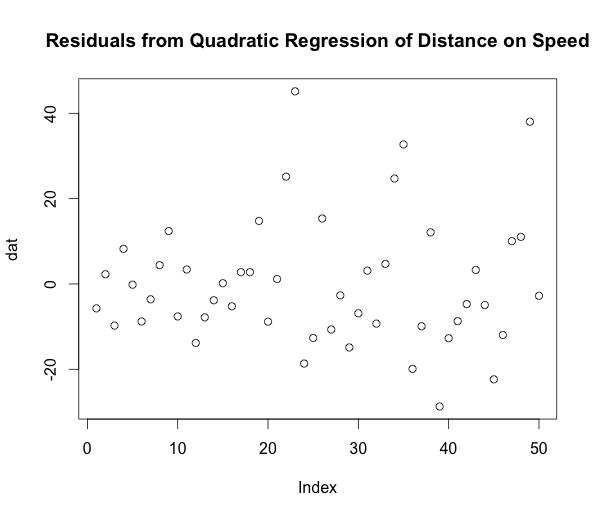
\includegraphics[scale=0.5]{Rplot1}
			\end{figure}
		\end{enumerate}
		I ran a two sample t-test using the two groups and obtained the output 
		\begin{verbatim}
				Welch Two Sample t-test

data:  y by z
t = -0.30353, df = 46.117, p-value = 0.7628
alternative hypothesis: true difference in means is not equal to 0
95 percent confidence interval:
 -9.829004  7.252954
sample estimates:
mean in group 0 mean in group 1 
     -0.6440125       0.6440125 

		\end{verbatim}
		Comparing this with the LMM framework, I used the nlme package with the formula \begin{verbatim}
			lme(fixed=y ~ z, random=~z|id, data=dat2)
		\end{verbatim}
		and obtained output
		\begin{verbatim}
Linear mixed-effects model fit by maximum likelihood
 Data: dat2 
       AIC      BIC    logLik
  421.6342 433.1063 -204.8171

Random effects:
 Formula: ~z | id
 Structure: General positive-definite, Log-Cholesky parametrization
            StdDev    Corr  
(Intercept) 15.582656 (Intr)
z           12.919203 -0.631
Residual     4.113828       

Fixed effects: y ~ z 
                 Value Std.Error DF    t-value p-value
(Intercept) -0.6440125  3.289774 48 -0.1957619  0.8456
z            1.2880249  4.243429 48  0.3035340  0.7628
 Correlation: 
  (Intr)
z -0.775

Standardized Within-Group Residuals:
        Min          Q1         Med          Q3         Max 
-0.46059391 -0.18826884 -0.04916520  0.08840635  1.06194027 

Number of Observations: 50
Number of Groups: 50 
		\end{verbatim}
	Under the fixed effects, we find the $t$-value in the slope agreeing (up to a sign since we're squaring) with the two sample t-test and producing identical p-values. We need to verify that
	\[
		\frac{\widehat{\beta}_1}{\mathrm{se}(\widehat{\beta}_1)} = \frac{\overline{X}_1 - \overline{X}_2}{\sqrt{\frac{s_1^2}{n_1} + \frac{s_2^2}{n_2}}}
	\]
	always holds under this type of model. Recall the likelihood in (a), which now takes the simpler form with $X_i^T = (1,z_i)^T$ and only four parameters $\sigma_1^2, \sigma_2^2, \beta_0,\beta_1$. The likelihood is
	\[
		\ell = -\frac{n_1+n_2}{2}\log(2\pi) -\frac{n_1}{2}\log\sigma_{1}^2 -\frac{n_2}{2}\log\sigma_{2}^2-\sum_{i=1}^{n_1}\frac{1}{2\sigma_{1}^2}(y_{i1} - \beta_0)^2 - \sum_{i=1}^{n_2} \frac{1}{2\sigma_2^2} (y_{i2} - \beta_0 -\beta_1)^2
	\]
	The derivatives are
	\begin{align*}
		\pd{\ell}{\sigma_1^2} &= -\frac{n_1}{2\sigma_1^2} + \frac{1}{2\sigma_1^4}\sum_{i=1}^{n_1} (y_{i1} - \beta_0)^2 \\
		\pd{\ell}{\sigma_2^2} &= -\frac{n_2}{2\sigma_2^2} + \frac{1}{2\sigma_2^4}\sum_{=1}^{n_2} (y_{i2} - \beta_0 - \beta_1)^2 \\
		\pd{\ell}{\beta_0} &= \sum_{i=1}^{n_1}\frac{1}{\sigma_{1}^2}(y_{i1} - \beta_0) + \sum_{i=1}^{n_2} \frac{1}{\sigma_2^2} (y_{i2} - \beta_0 -\beta_1)\\
		\pd{\ell}{\beta_1} &=   \sum_{i=1}^{n_2} \frac{1}{\sigma_2^2} (y_{i2} - \beta_0 -\beta_1)
	\end{align*}
	I do not see a way in this case to simultaneously solve for the variances, but I might be missing something obvious. I know we get $\widehat{\beta}_1 = \overline{X}_1 - \overline{X}_2$ in this case just from the output of LME and looking at the separate means produced in the t output. Therefore the denominators have to also be equal.
	\\ \\ It could also be the case that they're just very close, but again, I'm not sure.
\end{enumerate}
\newpage
R code
\begin{verbatim}
	setwd("~/Dropbox/UW2015-2016/Win2016/571/hw7")

dat <- read.table("dyestuff.txt", header = T)

wide = reshape(dat, timevar = "rep", idvar = "batch", direction = "wide")
wide <- wide[,-1]

m = 5
n = 6
mu = mean(dat[, 1]) #grand mean
Yibar <- apply(wide, 1, mean) #cluster means

f = m/(n-1)*sum((Yibar - mu)^2)*n*(m-1)/sum((wide-Yibar)^2)
1-pf(f,n-1, n*(m - 1))


library(nlme)
m1 <- lm(dist~speed+I(speed^2), data=cars)
dat = m1$residuals
dat2 = data.frame(dat,rep(c(1,0),each=25),1:50)
names(dat2) = c('y', 'z', 'id')
t.test(formula=y~z, data=dat2)
summary(fm1 <- lme(fixed=y ~ z, random=~z|id, data=dat2,method='ML'))

\end{verbatim}
\end{document}



